\documentclass[11pt,a4paper,titlepage]{article}
\usepackage{amsmath,amssymb,amstext,amsfonts,mathrsfs,graphicx}
\begin{document}
\title{GEP Protokoll - Laborversuch 5\\
Oszilloskop 2}
\author{Cao Thi Huyen \and Robert R\"osler \and Nico Grimm}
\date{7. Dezember 2015}
\maketitle
\section{Scheinwiderstandsmessung}
Mit einem Oszilloskop ist durch gleichzeitige Strom- und Spannungsmessung eine komplexe Impedanz \((\underline{Z}=R+j\omega L)\) einer Spule (0.1H, 10$\Omega$) zu bestimmen.
\subsection{Messaufbau}
Um den Spulenstrom mit dem Oszillioskop messen zu k\"onnen, wird der Spule ein geeigneter Widerstand (50$\Omega$) vorgeschaltet. Der Strom wird dann indirekt \"uber den Spannungsabfall an diesem Vorwiderstand bestimmt. Am Signalgenerator wird eine Frequenz von 50Hz (Sinus) eingestellt.
\begin{center}
Platzhalter f\"ur den Schaltplan
\end{center}
\subsection{Ergebnisse}
\subsubsection{Dokumentation der Zeitfunktionen von Strom und Spannung in DC-Kopplung}

\begin{center}
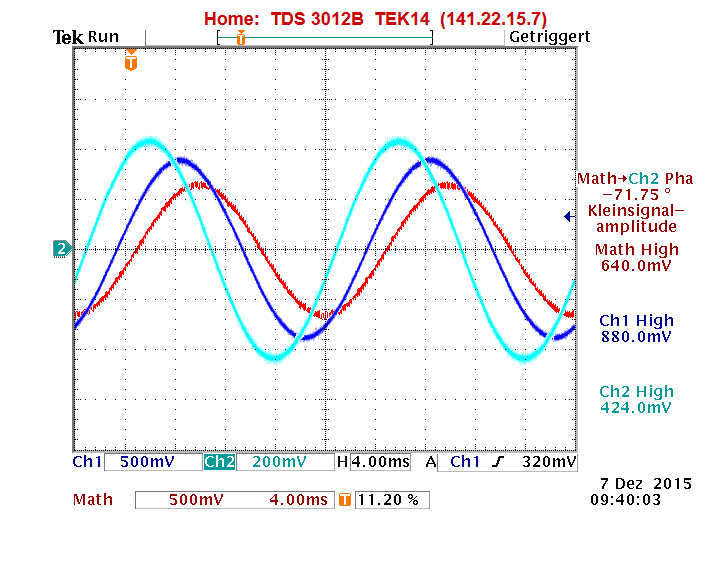
\includegraphics[width=0.9\textwidth]{5_1_1}
\end{center}
Channel 1 (hier dunkelblau) stellt die Spannung dar, die \"uber dem Vorwiderstand abf\"allt. Channel 2 (hier hellblau) stellt die Spannung \"uber der Spule dar. Der Gesamtstrom der flie\ss{}t, wird durch die Subtraktion von Channel 2 und Channel 1 rechnerisch dargestellt.
\newpage
\subsubsection{Berechnung der Impedanz \underline{Z} und Bestimmung der Bauelementgr\"o\ss{}en}

\newpage
\section{Messung der Kennlinie eines VDR im X-Y-Betrieb}
text
\end{document}
